\chapter{矢量分析}

\section {矢量代数}
\begin{enumerate}
	\item 
		\begin{eqnarray}
		&\vec{A} \cdot \vec{B} = AB\cos\theta& \\
		&\vec{A}\bot\vec{B}\Rightarrow\vec{A}\cdot\vec{B}=0& \\
		&\vec{A}\parallel\vec{B}\Rightarrow\vec{A}\cdot\vec{B}=AB&
		\end{eqnarray}
	\item 
		\begin{eqnarray}
		&\vec A \times \vec B = {\vec e_n}AB\sin \theta& \\
		&\vec A \times \vec B = \left|\begin{array}{ccc}
									    \vec e_x & \vec e_y & \vec e_z  \\ 
										A_x & A_y & A_z  \\
										B_x & B_y & B_z
									\end{array} \right|& \\
		&\vec{A}\bot\vec{B} \Rightarrow \left| \vec{A} \times \vec{B} \right|= AB& \\
		&\vec{A}\parallel\vec{B} \Rightarrow \left| \vec{A} \times \vec{B} \right|= 0& \\
		&\vec{A}\cdot (\vec{B}\times \vec{C})=\vec{B}\cdot (\vec{C}\times \vec{A})=\vec{C}\cdot (\vec{A}\times \vec{B})& \\
		&\vec{A}\times (\vec{B}\times \vec{C})=(\vec{A}\cdot \vec{C})\vec{B}-(\vec{A}\cdot \vec{B})\cdot \vec{C}&
		\end{eqnarray}
		
\end{enumerate}
\section{三种常用的正交曲线坐标系}
\begin{enumerate}
	\item 直角坐标系 图\ref{fig:zhijiao}
	\item 圆柱坐标系 图\ref{fig:yuanzhu}
	\item 球坐标系	图\ref{fig:qiu}
		\begin{figure}
			\centering
			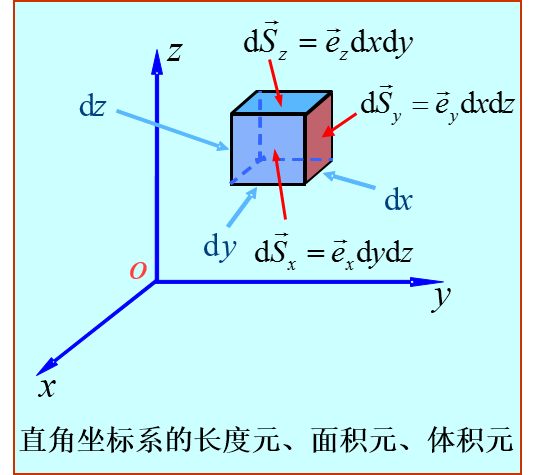
\includegraphics[keepaspectratio]{pics/直角坐标系}
			\caption{直角坐标系}
			\label{fig:zhijiao}
		\end{figure}
		\begin{figure}
			\centering
			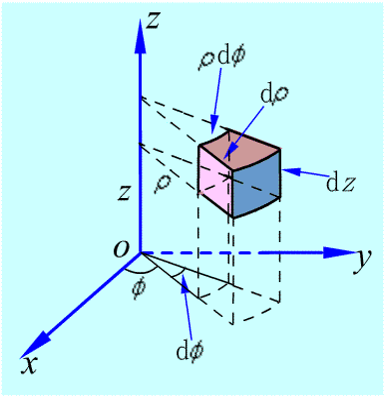
\includegraphics[keepaspectratio]{pics/圆柱坐标系}
			\caption{圆柱坐标系}
			\label{fig:yuanzhu}
		\end{figure}
		\begin{figure}
			\centering
			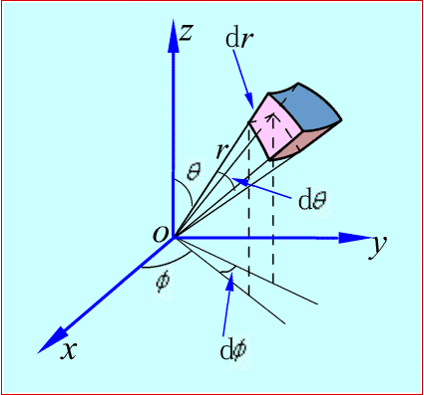
\includegraphics[keepaspectratio]{pics/球坐标系}
			\caption{球坐标系}
			\label{fig:qiu}
		\end{figure}
\end{enumerate}

\section{标量场的梯度}
\begin{enumerate}
	\item 方向导数
		\begin{eqnarray}
		&\frac{{\partial u}}{{\partial l}}\mathop |\nolimits_{{M_0}}  = \mathop {{\rm{lim}}}\limits_{\Delta l \to 0} \frac{{\Delta u}}{{\Delta l}} = \frac{{\partial u}}{{\partial x}}{\rm{cos}}\alpha  + \frac{{\partial u}}{{\partial y}}{\rm{cos}}\beta  + \frac{{\partial u}}{{\partial z}}{\rm{cos}}\gamma&
		\end{eqnarray}
	\item 梯度
		\begin{eqnarray}
		&\nabla u = {\vec e_x}\frac{{\partial u}}{{\partial x}} + {\vec e_y}\frac{{\partial u}}{{\partial y}} + {\vec e_z}\frac{{\partial u}}{{\partial z}}&
		\end{eqnarray}
\end{enumerate}

\section{矢量场的通量与散度}
\begin{enumerate}
	\item 通量
		\begin{eqnarray}
		&\psi  = \int {{\rm{d}}\psi  = } \int_S {\vec F \cdot {\rm{d}}\vec S}  = \int_S {\vec F \cdot {{\vec e}_n}{\rm{d}}S}&
		\end{eqnarray}
	\item 散度
		\begin{eqnarray}
		&\nabla  \cdot \vec F(x,y,z) = \mathop {\lim }\limits_{\Delta V \to 0} \frac{{\oint_S {\vec F(x,y,z) \cdot {\rm{d}}\vec S} }}{{\Delta V}}& \\
		&\nabla  \cdot \vec F = \frac{{\partial {F_x}}}{{\partial x}} + \frac{{\partial {F_y}}}{{\partial y}} + \frac{{\partial {F_z}}}{{\partial z}}&
		\end{eqnarray}
\end{enumerate}

\section{矢量场的环流和旋度}
\begin{enumerate}
	\item 环流
		\begin{eqnarray}
		&\Gamma  = \oint_C {\vec F(x,y,z) \cdot {\rm{d}}\vec l}	&
		\end{eqnarray}
	\item 环流面密度
		\begin{eqnarray}
		&{\rm{ro}}{{\rm{t}}_n}\vec F = \lim\limits_{\Delta S \to 0} \frac{1}{{\Delta S}}\oint_C {\vec F \cdot {\rm{d}}\vec l}	&
		\end{eqnarray}
	\item 旋度
		\begin{eqnarray*}
		&&{\rm{ro}}{{\rm{t}}_n}\vec F = {\vec e_n} \cdot \nabla  \times \vec F \\
		\nabla  \times \vec F&=&{\vec e_n}{[{\rm{ro}}{{\rm{t}}_n}\vec F]_{\max }} \\
		&=&{{\vec e}_x}\left( {{{\partial {F_z}} \over {\partial y}} - {{\partial {F_y}} \over {\partial z}}} \right) + {{\vec e}_y}\left( {{{\partial {F_x}} \over {\partial z}} - {{\partial {F_z}} \over {\partial x}}} \right) + {{\vec e}_z}\left( {{{\partial {F_y}} \over {\partial x}} - {{\partial {F_x}} \over {\partial y}}} \right) \\
		&=&\left| \begin{array}{ccc}
					{{{\vec e}_x}} & {{{\vec e}_y}} & {{{\vec e}_z}}  \\
					{{\partial  \over {\partial x}}} & {{\partial  \over {\partial y}}} & {{\partial  \over {\partial z}}} \\
					{{F_x}} & {{F_y}} & {{F_z}} 
					\end{array} \right|
		\end{eqnarray*}
	\item  两个恒等式
		\begin{eqnarray}
		&\nabla  \cdot (\nabla  \times \vec F) \equiv 0& \\
		&\nabla  \times (\nabla u) \equiv 0&
		\end{eqnarray}
	\item Stocks 定理
		\begin{eqnarray}
		&\oint_{{\kern 1pt} C} {{\kern 1pt} \vec F \cdot {\rm{d}}\vec l}  = \int_{{\kern 1pt} S} {{\kern 1pt} \nabla  \times \vec F \cdot {\rm{d}}\vec S}&
		\end{eqnarray}
\end{enumerate}

\section{拉普拉斯运算与格林定理}
\begin{enumerate}
	\item 格林定理(第一条是第一定理,后两条是第二定理)
	\begin{eqnarray}
	&\int_{V} (\nabla \Psi  \cdot \nabla \Phi  + \Psi {\nabla ^2}\Phi ){\rm{d}}V}  = \oint_{S} {(\Psi \nabla \Phi ) \cdot {\rm{d}}\vec S & \\
	&\int_{V} (\Psi {\nabla ^2}\Phi  - \Phi {\nabla ^2}\Psi ){\rm{d}}V}  = \oint_{S} {(\Psi \nabla \Phi  - \Phi \nabla \Psi ) \cdot {\rm{d}}\vec S& \\
	&\int_{V} (\Psi {\nabla ^2}\Phi  - \Phi {\nabla ^2}\Psi ){\rm{d}}V}  = \oint_{S} {(\Psi {{\partial \Phi } \over {\partial n}} - \Phi {{\partial \Psi } \over {\partial n}}){\rm{d}}S&
	\end{eqnarray}
\end{enumerate}

\section{亥姆霍兹定理}
\begin{enumerate}
	\item 亥姆霍兹定理
	\begin{eqnarray}
	&\vec F(\vec r) =  - \nabla u(\vec r) + \nabla  \times \vec A(\vec r)& \\
	&u(\vec r) = {1 \over {4{\rm{\pi }}}}\int_{{\kern 1pt} V} {{{\nabla ' \cdot \vec F(\vec r')} \over {\left| {\vec r - \vec r'} \right|}}} {\rm{d}}V'& \\
	&\vec A(\vec r) = {1 \over {4{\rm{\pi }}}}\int_{{\kern 1pt} V} {{{\nabla ' \times \vec F(\vec r')} \over {\left| {\vec r - \vec r'} \right|}}{\rm{d}}V'} &
	\end{eqnarray}
\end{enumerate}
